\documentclass[
    % twoside,
    a4paper,
    11pt,
    footinclude,
    % 12pt,
    DIV=11,
    english,
]{scrreprt}
\usepackage{scrhack} % NOTE: fix some KOMA warnigns
\usepackage[english]{babel}
\usepackage[utf8]{inputenc}
\usepackage[T1]{fontenc}



%% adapt for printing
\usepackage[
    a4paper,
    pdftex,
    % inner=30mm,
    % outer=30mm,
    % vmargin=30mm,
    % bindingoffset=0mm
]{geometry}

%% acronyms and glossary
\usepackage[
    single=true,
    sort=true,
    only-used=true
]{acro}

\setlength{\marginparwidth}{2cm}

%% comments for reviews
\usepackage{amssymb}% http://ctan.org/pkg/amssymb
\usepackage{pifont}% http://ctan.org/pkg/pifont

% PDF inclusion
\usepackage{pdflscape}
\usepackage[final]{pdfpages}

%% figures, diagrams, and plots
\usepackage{graphicx}
\usepackage{tikz}
\usepackage{pgfplots}
\usepackage{tabulary}
\usepackage{svg}
\usepackage{amsmath}

%% Subfigure for ordering multiple pictures in one figure scope
\usepackage{subfigure}

%% Figure placement
\usepackage{float} % use H option to force placement

%% used for bytefields
\usepackage{bytefield}
\usepackage{rotating}

\pgfplotsset{compat=newest}
\pgfplotsset{compat=1.9}
\usepgfplotslibrary{colorbrewer}

%% tables
\usepackage{booktabs}
\usepackage{tabularx}

%% units & Symbols
\usepackage{siunitx}
\usepackage{textcomp} % Fix undefined symbols warnings for gensymb, see https://latex.org/forum/viewtopic.php?f=4&t=3364#p13124
\usepackage{gensymb}

%% unifying quote marks when using different languages
%% NOTE: Fixes warning concerning polyglossia when including biblatex
\usepackage{csquotes}

%% bibliography
\usepackage[]{biblatex}
\addbibresource{bibliography.bib}

%% head- and footlines
\usepackage{scrlayer-scrpage}
\setkomafont{pagehead}{\normalfont\small\sffamily}
\setkomafont{pagefoot}{\small}
\setkomafont{pagenumber}{\normalfont\bfseries}

\automark[chapter]{chapter}
%\automark[section]{section}

\ihead{}
\chead{}
\ohead{\headmark}
\ifoot*{}
\cfoot*{}
\ofoot*{\pagemark}

% special chapter mark
\renewcommand{\chaptermark}[1]{%
    \markboth{%
        \MakeUppercase{%
            \chapapp%
        }%
        \thechapter%
        $\bigl{|}$~%
        \textcolor{black}{%
            \MakeUppercase{%
                % \so{%
                    #1%
                % }%
            }%
        }%
    } {%
        \textcolor{black}{%
            \MakeUppercase{%
                % \so{%
                    #1%
                % }%
            }%
        }%
        $\bigl{|}$~%
        \MakeUppercase{%
            \chapapp%
        }%
        \thechapter%
    }%
}

% no indent at start of paragraphs
\parindent 0pt

% disable extra space after colon
\frenchspacing

%% hyperref
\usepackage{hyperref}
\hypersetup{
    hidelinks,
    breaklinks=true,
    pdfpagemode=UseNone,
    pageanchor=true,
    pdfpagemode=UseOutlines,
    plainpages=false,
    bookmarksnumbered=true,
}

\usepackage{graphicx}
\begin{document}
\pagestyle{plain}%
\pagenumbering{roman}

\begin{titlepage}
    \begin{figure}[!tbp]
        \centering
        \begin{minipage}[b]{0.55\linewidth}
            
\includegraphics[height=2cm]{pictures/HTWG_logo.png}
        \end{minipage}%
        \hfill%
        \begin{minipage}[b]{0.4\linewidth}
            \hfill%
            %
\includegraphics[height=2cm]{pictures/HTWG_logo.png}
        \end{minipage}%
    \end{figure}
    \centering
    {\scshape\Large HTWG - Hochschule für Technik, Wirtschaft und Gestaltung \par}
    \vspace{1cm}
    {\scshape\LARGE Masterprojektarbeit\par}
    \vspace{1.5cm}
    {\huge\bfseries User Guide UWB GUI\par}
    \vspace{2cm}
    {\Large Positionsbestimmung mittels Ultrabreitband \par}
    \vfill
    erstellt von\par
    Tom \textsc{Herter}\par
    EIM 3\par
    Mtr. 306971\par
    \&\par
    Sebastian \textsc{Krebs}\par
    EIM 3\par
    Mtr. 298229\par
    \vfill
    betreut durch\par
    Prof.\ Dr.~\textsc{Knievel}
    \vfill
% Bottom of the page
	{\large Konstanz, \today\par}
\end{titlepage}



%\cleardoublepage%
%\begingroup
    \let\clearpage\relax            % disable \clearpage
    \let\cleardoublepage\relax      % disable \cleardoublepage

    \chapter*{Zusammenfassung}
    \pdfbookmark[1]{Zusammenfassung}{Zusammenfassung}
    \fontsize{10}{12}\selectfont

    XXX
    % back of abstract page
    \vfill
    \newpage
    \thispagestyle{empty}
    ~\vfill
\endgroup           % enables \clearpage and \cleardoublepage again


%\cleardoublepage%
%\begingroup
    \let\clearpage\relax        % disable \clearpage
    \let\cleardoublepage\relax  % disable \cleardoublepage

    \pdfbookmark[1]{Eidesstattliche Erklärung}{Eidesstattliche Erklaerung}
    \chapter*{Eidesstattliche Erklärung}

    Ich erkläre hiermit an Eides statt, dass ich die vorliegende Arbeit selbständig verfasst
    und dabei keine anderen als die angegebenen Hilfsmittel benutzt habe.
    Sämtliche Stellen der Arbeit, die im Wortlaut oder dem Sinn nach Publikationen
    oder Vorträgen anderer Autoren entnommen sind, habe ich als solche kenntlich gemacht.
    Die Arbeit wurde bisher weder gesamt noch in Teilen einer anderen Prüfungsbehörde
    vorgelegt und auch noch nicht veröffentlicht.\par
    \vspace{2cm}

    \begin{minipage}[h]{0.4\linewidth}
        \begin{center}
            Karlsruhe, den \today\par
            \dotfill\\
            (Ort, Datum)
            \vspace*{2.5mm}
        \end{center}
    \end{minipage}%
    \hfill%
    \begin{minipage}[h]{0.5\linewidth}
        \begin{center}
            \vspace*{5.5mm}
            \dotfill\\
            (Unterschrift)
            \vspace*{2.5mm}
        \end{center}
    \end{minipage}%

    \vfill
    % Yardeye Disclaimer
    Die vorliegende Arbeit stellt mein persönliches Arbeitsergebnis dar und ist kein offizielles Dokument der Yardeye GmbH.

    % back of acknowledgement page
    \vfill
    \newpage
    \thispagestyle{empty}
    \vfill

\endgroup   % enable \clearpage and \cleardoublepage again


%\cleardoublepage%

\tableofcontents%
\pagebreak%

\setcounter{section}{0}
\pagestyle{headings}%
\pagenumbering{arabic}%
\setcounter{tocdepth}{1}
\setcounter{secnumdepth}{2} % default value for 'report' class is "2"

{\let\clearpage\relax \chapter{Introduction}

\section{Description}

This software guide is designed to explain the concept of the firmware running on the UWB tag and all the UWB anchor devices. 
The goal is to give a understanding what classes and files are used and how the interoperate together. 
Additionally to this guide a fill Doxygen documentation will be provided. 

\section{Naming Conventions}
Within this Software Guide detailing the Time-of-Flight (TOF) function, it's important to note that the terms "initiator" and "tag" are used interchangeably. 
Both refer to the UWB (Ultra-Wideband) device responsible for initiating the TOF measurement by transmitting a UWB request to the relevant devices in its vicinity.

These devices can also be alternatively referred to as "anchor", "responder" or "landmark". This nomenclature is employed because these devices play the pivotal role of responding to the UWB request and guiding the initiator in computing the distance between them. The interchangeable use of these terms is intended to provide clarity and flexibility in describing the dynamic roles these devices undertake in the TOF measurement process.

\section{Basic functionality and setup}
The primary function of this setup revolves around the estimation of tag positions within a predefined coordinate space. 
This estimation is achieved by leveraging the distances between the tag and various anchors strategically placed within the room. 
To facilitate a clearer grasp of the setup's workings, an illustrative sketch featuring example coordinates can be found in Figure \ref{fig:setup_sketch}.
\vspace{4pt}
\newline
In this setup, the anchors are situated throughout the room in a deliberate yet arbitrary manner, each possessing known coordinates. 
The key to this system's functionality lies in the tag device's ability to discern the positions of these anchors. 
With this information, the tag can deduce its own location in all the X, Y and Z directions by gauging the distances to all the anchors.
\vspace{4pt}
\newline
In Figure \ref{fig:setup_sketch}, these distances are visually represented and labeled as d\_1 to d\_5. 
The critical aspect of this process is that it enables the tag device to employ an Extended Kalman Filter (EKF) for the purpose of position estimation. 
This filter algorithm plays a pivotal role in refining and enhancing the accuracy of the tag's estimated position within the coordinate space and is further discussed in chapter \ref{chap:EKF_Handling}. 

\begin{figure}[!hbt]
	\centering
	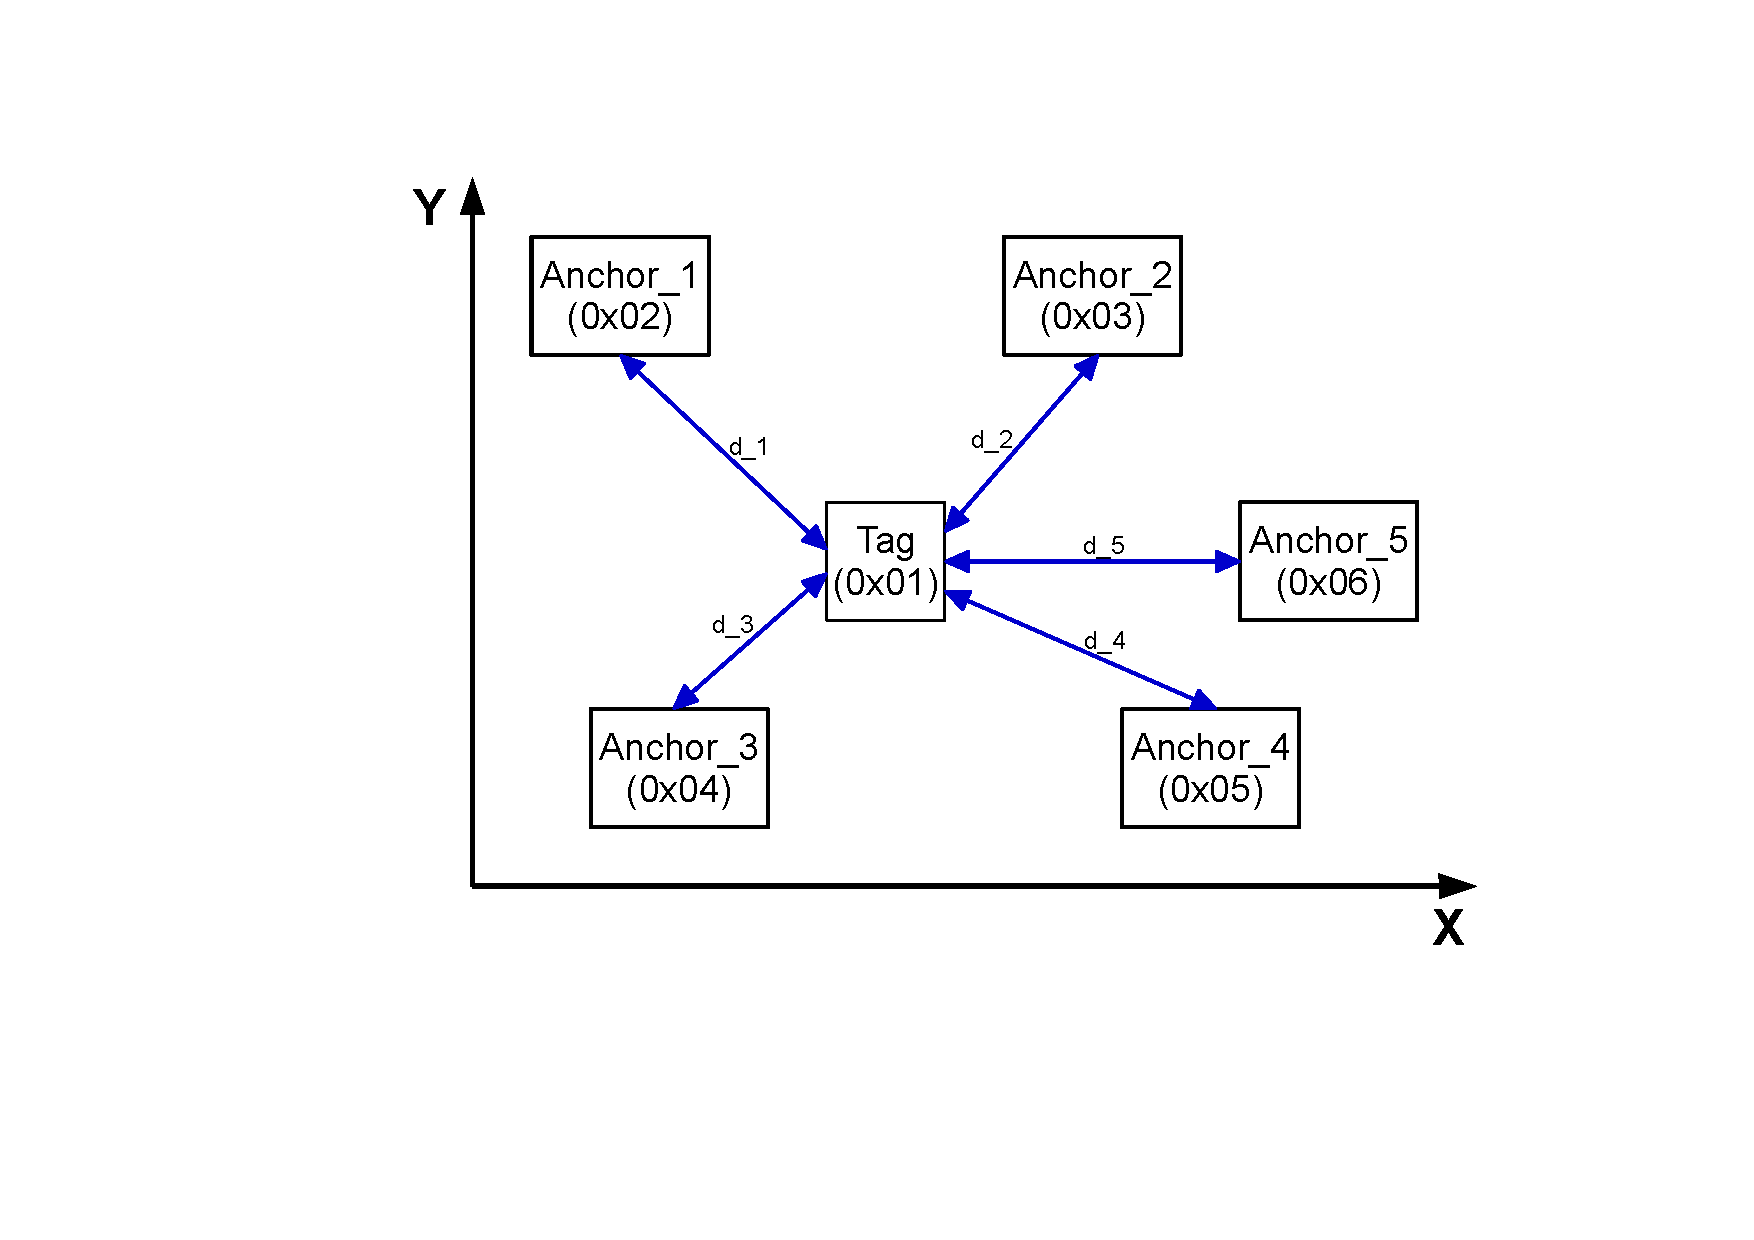
\includegraphics[width=0.6\textwidth]{pictures/Complete_Setup.pdf}
	\caption{Sketch of the complete setup.}
	\label{fig:setup_sketch}
\end{figure}

\section{Flow of Information}

In Figure \ref{fig:information_flow} the information flow of the entire system is pictured. 
The most important component are the UWB ranging messages exchanged between the Tag and every Anchor that are ultimately used to estimate the Tag's position. 
With every sent UWB message from the Tag to an Anchor the channel parameters are extracted and transmitted via WiFi to an MQTT-Server. 
The UWB Tag itself also transmits its coordinates over MQTT to a different topic. 
The MQTT mechanics are further discussed in \ref{chap:MQTT_Handling}. 
\vspace{4pt}
\newline
The configuration of the Tag, meaning putting in the coordinate of each anchor to the EEPROM, is executed via Bluetooth by a Bluetooth-Capable device running the configuration software. 
Additionally the Tag sends its position via Bluetooth where the configuration software has the ability to display it in a 2D plot in real time. 
Bluetooth Handling techniques are further elaborated in \ref{chap:Bluetooth_Handling}. 

\begin{figure}[!hbt]
	\centering
	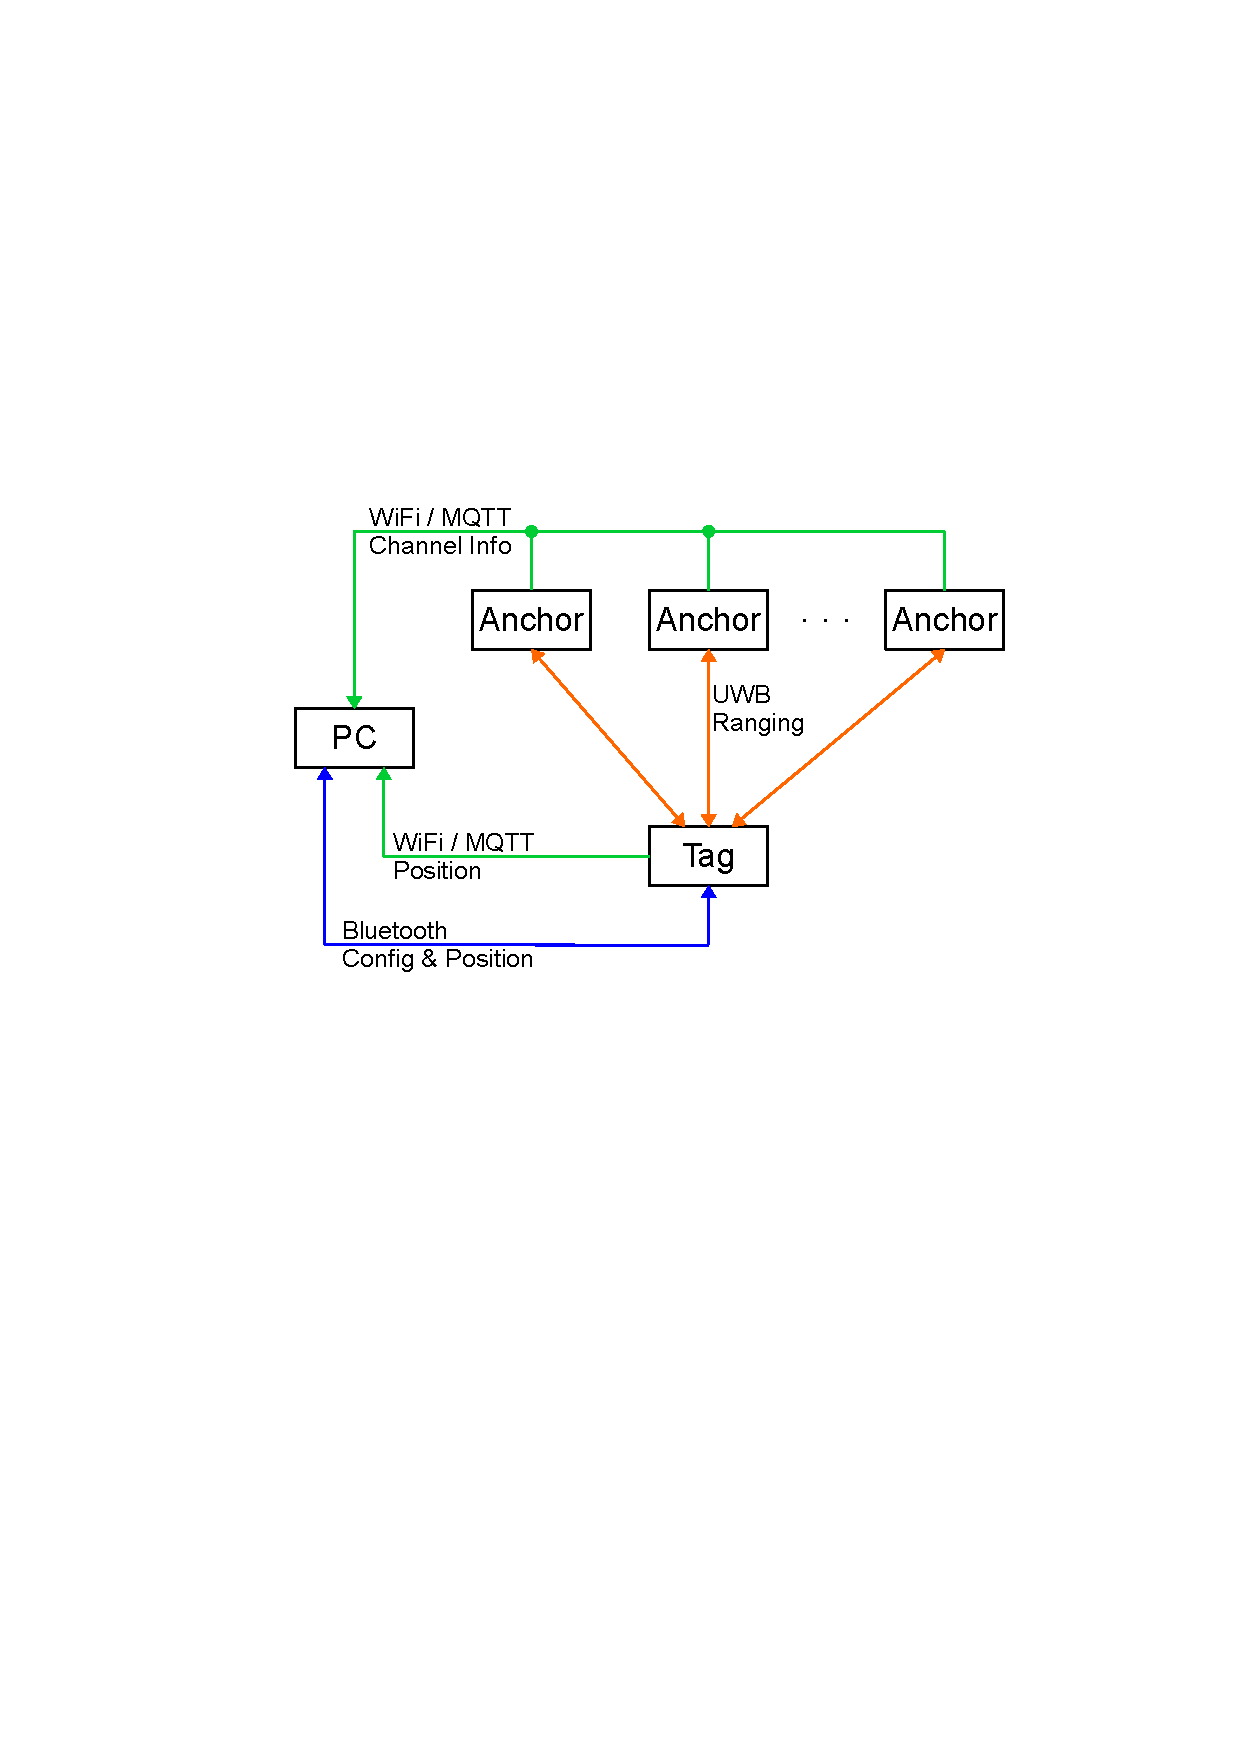
\includegraphics[width=0.6\textwidth]{pictures/information_flow.pdf}
	\caption{Sketch of the complete setup.}
	\label{fig:information_flow}
\end{figure}












}
{\let\clearpage\relax \chapter{Hardware Requirements}

Before you can establish a connection with the UWB Tag, ensure that your computer has a built-in Bluetooth adapter or an external Bluetooth dongle. Most modern laptops and desktops come equipped with Bluetooth capabilities. If your computer lacks built-in Bluetooth, you may need to purchase a compatible USB Bluetooth dongle, plug it into an available USB port and install corresponding driver software. 
Make sure that the device is recognised correctly in the device manager. 

When you run the file as an .exe on a Windows machine you do not need a Python 3 version to be installed. }
\chapter{Getting started}

When starting the Software for the first time you are set up with an empty dashboard. 
However you can plaace, resize or remove the widgeds individually and save/load your own instance of the dashboard. 


\begin{figure}[!hbt]
	\centering
	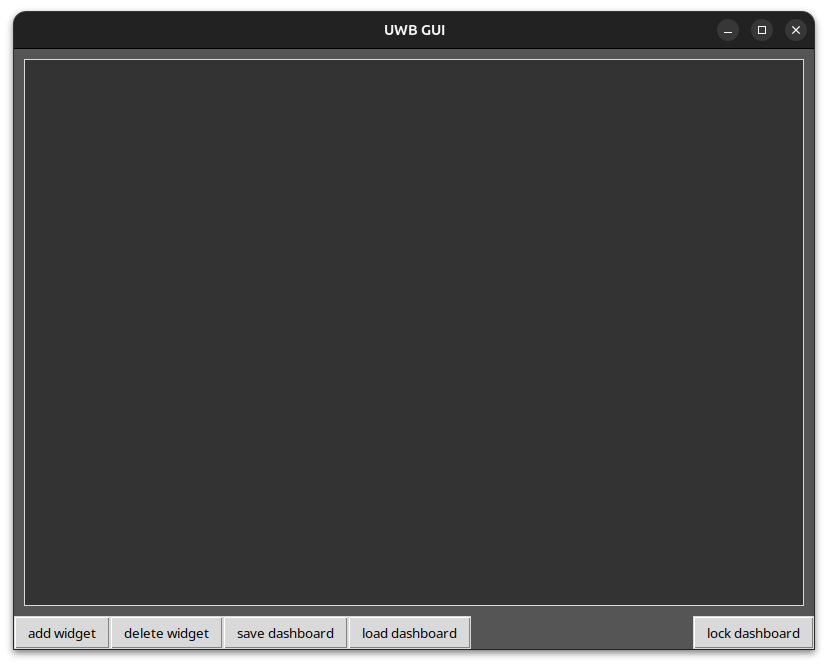
\includegraphics[width=0.65\textwidth]{pictures/gui_idle.png}
	\caption{Empty GUI after startup}
	\label{fig:gui_idle}
\end{figure}



\section{Add a Widget}
Adding a widget is a fundamental action in your dashboard application. Widgets are the building blocks of your dashboard, allowing you to display various types of information and functionality. To add a widget to your dashboard, follow these steps:

Click the "Add Widget" button: Locate and click the "add widget" button on your dashboard's user interface. This action will trigger a dialog or menu to appear like desplayed in Figure \ref{fig:add_widget}.

Select Widget Type: In the dialog or menu, you'll be presented with a list of available widget types. Choose the type of widget you want to add to your dashboard. Your options include "BleServiceWidget", "BleConfigWidget", "SerialWidget" and "BlePlotPositionWidget". 

Confirm and Add: Click the "OK" button to confirm your selection. The selected widget will now be added to your dashboard canvas.

Customize and Position: Once added, you can customize the widget's appearance and content as needed. You can also position it on the canvas by dragging it to your desired location.

Repeat as Needed: You can add multiple widgets to your dashboard following the same process. Each widget can serve a unique purpose and display distinct information.

\begin{figure}[!hbt]
	\centering
	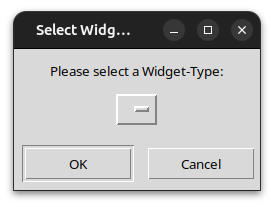
\includegraphics[width=0.35\textwidth]{pictures/add_widget.png}
	\caption{Prompt to add a widget}
	\label{fig:add_widget}
\end{figure}

\section{Remove a Widget}
If you no longer need a widget on your dashboard or wish to rearrange its layout, you can remove it. Here's how to remove a widget from your dashboard:

Click the "Remove Widget" Button: Locate and click the "delete widget" or "remove widget" button on your dashboard's user interface. This action will prompt a dialog or input box.

Specify Widget to Remove: In the dialog, you may need to specify which widget you want to remove. This is typically done by entering the widget's index or selecting it from a list.

Confirm Deletion: Confirm your choice to delete the widget. The selected widget will be removed from your dashboard, and the layout will adjust accordingly.

Optional: You can repeat this process to remove additional widgets as needed.

\begin{figure}[!hbt]
	\centering
	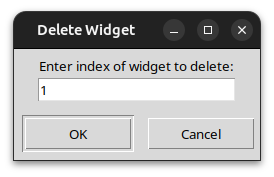
\includegraphics[width=0.35\textwidth]{pictures/delete_widget.png}
	\caption{Prompt to remove a widget}
	\label{fig:delete_widget}
\end{figure}


\section{Save Current Dashboard}
Saving your current dashboard layout and widget configurations allows you to preserve your work for future use. To save your current dashboard, follow these steps:

Click the "Save Dashboard" Button: Locate and click the "save dashboard" button on your dashboard's user interface. This action will initiate the saving process.

\section{Load a Dashboard}
Loading a previously saved dashboard configuration allows you to restore a layout and widget setup. Here's how to load a dashboard:

Click the "Load Dashboard" Button: Locate and click the "load dashboard" button on your dashboard's user interface. This action will load the last saved dashbord onto the user interface.

Continue Editing: You can continue editing and customizing your loaded dashboard as needed.

\section{Lock / Unlock Dashboard}
Locking and unlocking the dashboard is a feature that restricts or enables interaction with the widgets on the canvas. Here's how to lock and unlock your dashboard:

\subsection{Lock Dashboard}
Click the "Lock Dashboard" Button: Locate and click the "lock dashboard" button on your dashboard's user interface. This action will activate the dashboard lock feature.

Widgets Become Static: When the dashboard is locked, all widgets on the canvas become static and unresponsive to user interactions. You cannot move or resize them.

Limited Functionality: Some buttons or features for adding, removing, or configuring widgets may become disabled while the dashboard is locked like the add and remove widget buttons. 

\subsection{Unlock  Dashboard}
Click the "Unlock Dashboard" Button: To regain full interaction with your widgets, click the "unlock dashboard" button on your dashboard's user interface. This action will deactivate the dashboard lock feature.

Widgets Become Interactive: Once the dashboard is unlocked, you can freely move, resize, and interact with the widgets as needed.

Full Functionality Restored: All buttons and features related to widget management become active and usable when the dashboard is unlocked.

Use the lock and unlock feature as needed to control the level of interactivity and customization available for your widgets on the dashboard. This feature can be especially useful when you want to prevent accidental changes to your layout.
{\let\clearpage\relax \chapter{Widgets}

 
\section{BleConfigWidget}

The BleConfigWidget is a specialized widget in your dashboard application designed to interact with the tag device, retrieve configuration data from it, and update the configuration remotely. 

In order to view the current configuration and change it, go through the following steps. 

\begin{enumerate}
	\item Add the BleConfigWidget widget to your dashboard. Drag and resize it if needed. 
	\item On the Tag device hit the user button 1 and look for a change in the user LEDs. When the config mode is entered the should blink in a repetetive pattern. 
	\item Hit the "Refresh" button and wait for a few seconds for your device to scan the vicinity for Bluetooth devices. 
	\item Select the "ESP32" device from the device list right to the Refresh button. 
	\item Hit the "Connect" button. After a short time the saved coordinates for each anchor device. 
	\item To change the coordinates, define them in your setup physical by measuring thei position in relation to the origin (0,0,0). 
	\item Simpy change the already displayed coordinates. once the system noticed a change in a certain value the cell will change its color to red. 
	\item Once you are finished reconfigurating you need to hit the "Uplpoad" button below the displayed coordinates to transfer the new values to the tag device. 
	\item To initiate the saving process you hit the "Save Config". The Tag device will automatically update the values by writing them into its EEPROM and reboot. 
\end{enumerate}

\newpage

\begin{figure}[!hbt]
	\centering
	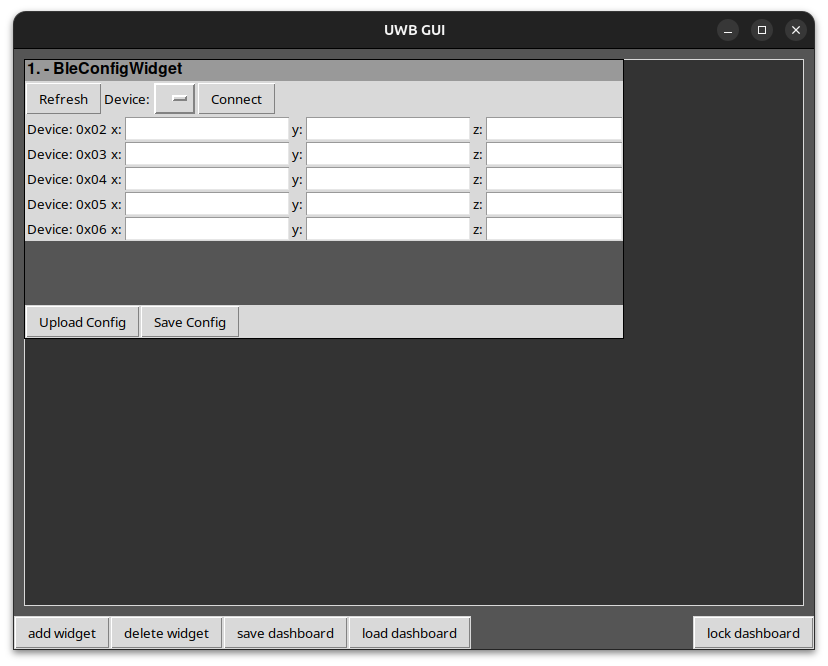
\includegraphics[width=0.42\textwidth]{pictures/cofig_device_idle.png}
	\caption{Empty configuration widget before connecting.}
	\label{fig:cofig_device_idle}
\end{figure}

\begin{figure}[!hbt]
	\centering
	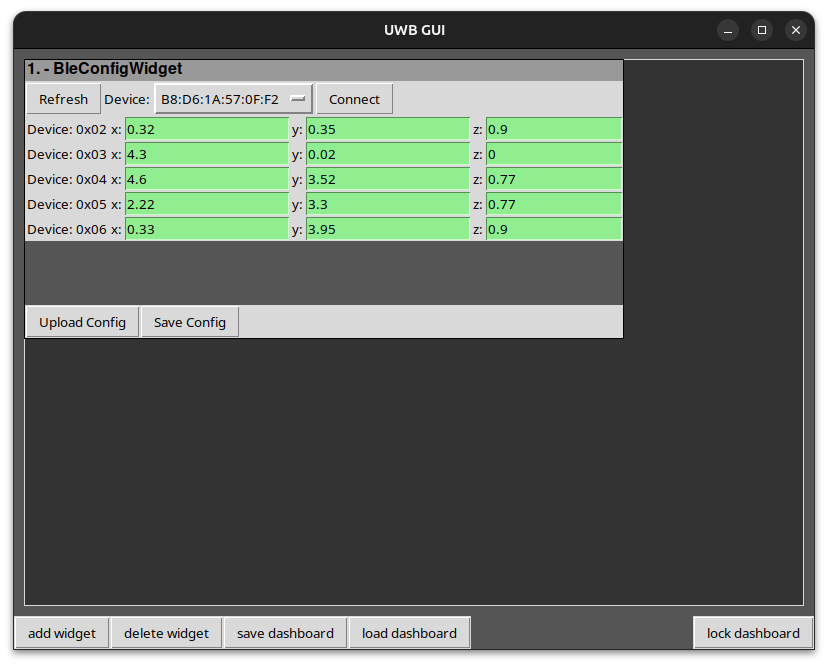
\includegraphics[width=0.42\textwidth]{pictures/config_device_connected.png}
	\caption{Configuration widget is displaying the currently saced coordinates after connecting successfully.}
	\label{fig:config_device_connected}
\end{figure}

\begin{figure}[!hbt]
	\centering
	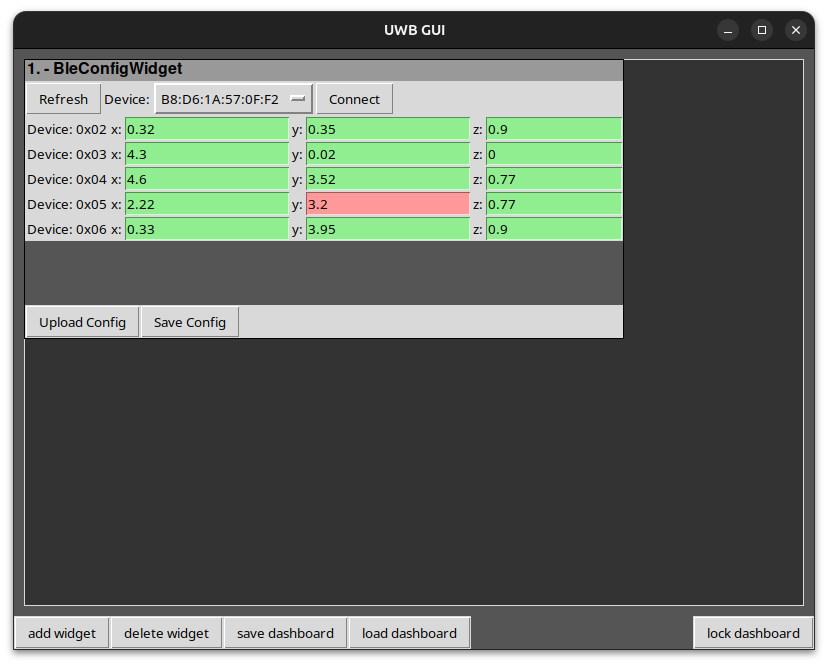
\includegraphics[width=0.42\textwidth]{pictures/config_coordinate_changed.png}
	\caption{Configuration widget is displaying the changed coordinate in red. }
	\label{fig:config_coordinate_changed}
\end{figure}

\newpage

\section{BlePlotPositionWidget}

The BlePlotPositionWidget lets you display the current position of the tag in the choosen coordinate system. 
In order to use it properly use it go through the following steps. 

\begin{enumerate}
	\item Add the BleConfigWidget widget to your dashboard. Drag and resize it if needed. 
	\item Make sure that all anchor devices 0x02 to 0x06 are up and running properly. Otherwise the estimated position may vary a lot. 
	\item Make sure the tag device is running and in uwb mode. That state is given if the LED 1 is consistently on and the green uwb RX and TX LEDs are blinking. 
	\item Hit the "Refresh" button and wait for a few seconds for your device to scan the vicinity for Bluetooth devices. 
	\item Select the "ESP32" device from the device list right to the Refresh button. 
	\item Hit the "Connect" button. After a short time the saved coordinates for each anchor device. 
	\item Now in the given plot of the widget a dot with the current estimated position is added. 
\end{enumerate}

\begin{figure}[!hbt]
	\centering
	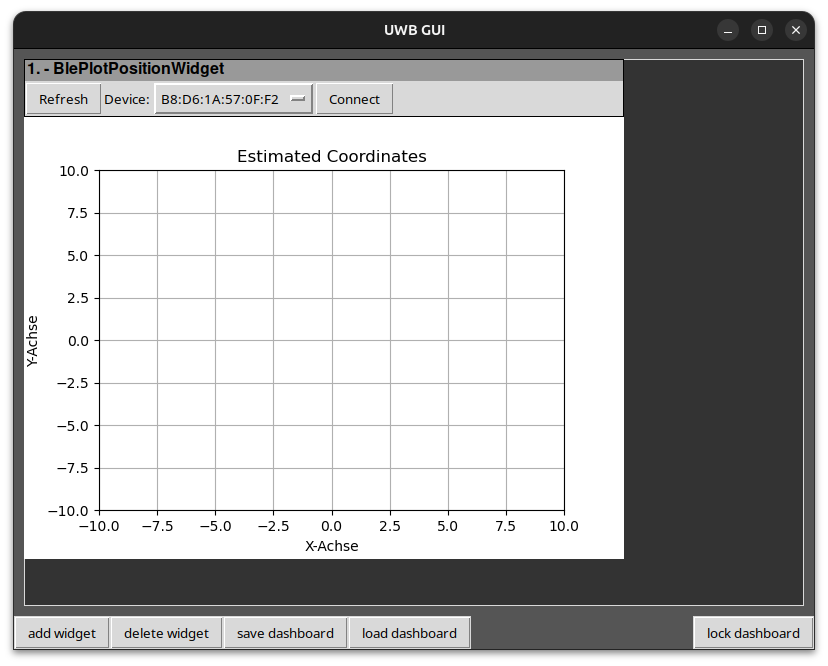
\includegraphics[width=0.6\textwidth]{pictures/coordinate_plot.png}
	\caption{Plot Position Widget with no position currently displayed.}
	\label{fig:coordinate_plot}
\end{figure}
}


\end{document}
